%\begin{figure}[H]
%    \tiny
%    \centering
%\resizebox{\textwidth}{!}{%}}
    \setlength{\tabcolsep}{.25pt}
    \begin{tabular}{cccccccccc}
        & \mr{2}{\tiny\Th{Input}} & \mc{2}{\tiny\Th{Grad-CAM}} & \mc{2}{\tiny\Th{Grad-CAM++}} & \mc{2}{\tiny\Th{Score-CAM}} & \mc{2}{\tiny\Th{Ablation-CAM}} \\
        & & \tiny\Th{Baseline} & \tiny\Th{Ours} & \tiny\Th{Baseline} & \tiny\Th{Ours} & \tiny\Th{Baseline} & \tiny\Th{Ours} & \tiny\Th{Baseline} & \tiny\Th{Ours} \\
    
         {\rotatebox{90}{\tiny \Th{Man}}} &
         
\includegraphics[width=.09\textwidth]{fig/gradient/fig/fig_cam/original/4862.JPEG} &
         \includegraphics[width=.09\textwidth]{fig/gradient/fig/fig_cam/baseline/gradcam/4862.JPEG} &
         \includegraphics[width=.09\textwidth]{fig/gradient/fig/fig_cam/cosine/gradcam/4862.JPEG} &
         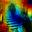
\includegraphics[width=.09\textwidth]{fig/gradient/fig/fig_cam/baseline/gradcampp/4862.JPEG} &
         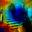
\includegraphics[width=.09\textwidth]{fig/gradient/fig/fig_cam/cosine/gradcampp/4862.JPEG} &
         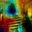
\includegraphics[width=.09\textwidth]{fig/gradient/fig/fig_cam/baseline/scorecam/4862.JPEG} &
         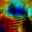
\includegraphics[width=.09\textwidth]{fig/gradient/fig/fig_cam/cosine/scorecam/4862.JPEG} &
         \includegraphics[width=.09\textwidth]{fig/gradient/fig/fig_cam/baseline/ablationcam/4862.JPEG} &
         \includegraphics[width=.09\textwidth]{fig/gradient/fig/fig_cam/cosine/ablationcam/4862.JPEG} \\
    
        {\rotatebox{90}{\tiny \Th{Girl}}} &
        
\includegraphics[width=.09\textwidth]{fig/gradient/fig/fig_cam/original/2641.JPEG} &
        
\includegraphics[width=.09\textwidth]{fig/gradient/fig/fig_cam/baseline/gradcam/2641.JPEG} &
        
\includegraphics[width=.09\textwidth]{fig/gradient/fig/fig_cam/cosine/gradcam/2641.JPEG} &
        
\includegraphics[width=.09\textwidth]{fig/gradient/fig/fig_cam/baseline/gradcampp/2641.JPEG} &
        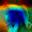
\includegraphics[width=.09\textwidth]{fig/gradient/fig/fig_cam/cosine/gradcampp/2641.JPEG} &
        
\includegraphics[width=.09\textwidth]{fig/gradient/fig/fig_cam/baseline/scorecam/2641.JPEG} &
        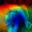
\includegraphics[width=.09\textwidth]{fig/gradient/fig/fig_cam/cosine/scorecam/2641.JPEG} &
        
\includegraphics[width=.09\textwidth]{fig/gradient/fig/fig_cam/baseline/ablationcam/2641.JPEG} &
        
\includegraphics[width=.09\textwidth]{fig/gradient/fig/fig_cam/cosine/ablationcam/2641.JPEG} \\
    
        {\rotatebox{90}{\tiny \Th{Woman}}} &
        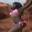
\includegraphics[width=.09\textwidth]{fig/gradient/fig/fig_cam/original/5257.JPEG} &
        \includegraphics[width=.09\textwidth]{fig/gradient/fig/fig_cam/baseline/gradcam/5257.JPEG} &
        \includegraphics[width=.09\textwidth]{fig/gradient/fig/fig_cam/cosine/gradcam/5257.JPEG} &
        
\includegraphics[width=.09\textwidth]{fig/gradient/fig/fig_cam/baseline/gradcampp/5257.JPEG} &
        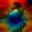
\includegraphics[width=.09\textwidth]{fig/gradient/fig/fig_cam/cosine/gradcampp/5257.JPEG} &
        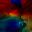
\includegraphics[width=.09\textwidth]{fig/gradient/fig/fig_cam/baseline/scorecam/5257.JPEG} &
        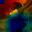
\includegraphics[width=.09\textwidth]{fig/gradient/fig/fig_cam/cosine/scorecam/5257.JPEG} &
        \includegraphics[width=.09\textwidth]{fig/gradient/fig/fig_cam/baseline/ablationcam/5257.JPEG} &
        \includegraphics[width=.09\textwidth]{fig/gradient/fig/fig_cam/cosine/ablationcam/5257.JPEG}\\
    
        {\rotatebox{90}{\tiny \Th{Lobster}}} &
        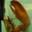
\includegraphics[width=.09\textwidth]{fig/gradient/fig/fig_cam/original/5160.JPEG} &
        \includegraphics[width=.09\textwidth]{fig/gradient/fig/fig_cam/baseline/gradcam/5160.JPEG} &
        \includegraphics[width=.09\textwidth]{fig/gradient/fig/fig_cam/cosine/gradcam/5160.JPEG} &
        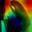
\includegraphics[width=.09\textwidth]{fig/gradient/fig/fig_cam/baseline/gradcampp/5160.JPEG} &
        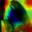
\includegraphics[width=.09\textwidth]{fig/gradient/fig/fig_cam/cosine/gradcampp/5160.JPEG} &
        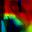
\includegraphics[width=.09\textwidth]{fig/gradient/fig/fig_cam/baseline/scorecam/5160.JPEG} &
        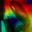
\includegraphics[width=.09\textwidth]{fig/gradient/fig/fig_cam/cosine/scorecam/5160.JPEG} &
        \includegraphics[width=.09\textwidth]{fig/gradient/fig/fig_cam/baseline/ablationcam/5160.JPEG} &
        \includegraphics[width=.09\textwidth]{fig/gradient/fig/fig_cam/cosine/ablationcam/5160.JPEG} \\
    
        {\rotatebox{90}{\tiny \Th{Couch}}} &
        
\includegraphics[width=.09\textwidth]{fig/gradient/fig/fig_cam/original/2043.JPEG} &
        \includegraphics[width=.09\textwidth]{fig/gradient/fig/fig_cam/baseline/gradcam/2043.JPEG} &
        \includegraphics[width=.09\textwidth]{fig/gradient/fig/fig_cam/cosine/gradcam/2043.JPEG} &
        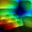
\includegraphics[width=.09\textwidth]{fig/gradient/fig/fig_cam/baseline/gradcampp/2043.JPEG} &
        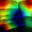
\includegraphics[width=.09\textwidth]{fig/gradient/fig/fig_cam/cosine/gradcampp/2043.JPEG} &
        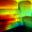
\includegraphics[width=.09\textwidth]{fig/gradient/fig/fig_cam/baseline/scorecam/2043.JPEG} &
        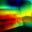
\includegraphics[width=.09\textwidth]{fig/gradient/fig/fig_cam/cosine/scorecam/2043.JPEG} &
        \includegraphics[width=.09\textwidth]{fig/gradient/fig/fig_cam/baseline/ablationcam/2043.JPEG} &
        \includegraphics[width=.09\textwidth]{fig/gradient/fig/fig_cam/cosine/ablationcam/2043.JPEG} \\
    \end{tabular}
%}
    %\vspace{3pt}
    %\caption{\textbf{Saliency map comparison} of standard \vs our training using different CAM-based methods on CIFAR-100 examples.}
    %\label{fig:salient}
    %\end{figure}